\documentclass[border=6pt]{standalone}
\usepackage{amsmath,amssymb}
\usepackage{tikz}
\usetikzlibrary{arrows.meta,calc,decorations.pathreplacing,decorations.markings,patterns,shapes.geometric,positioning,shadings,plotmarks}

\begin{document}
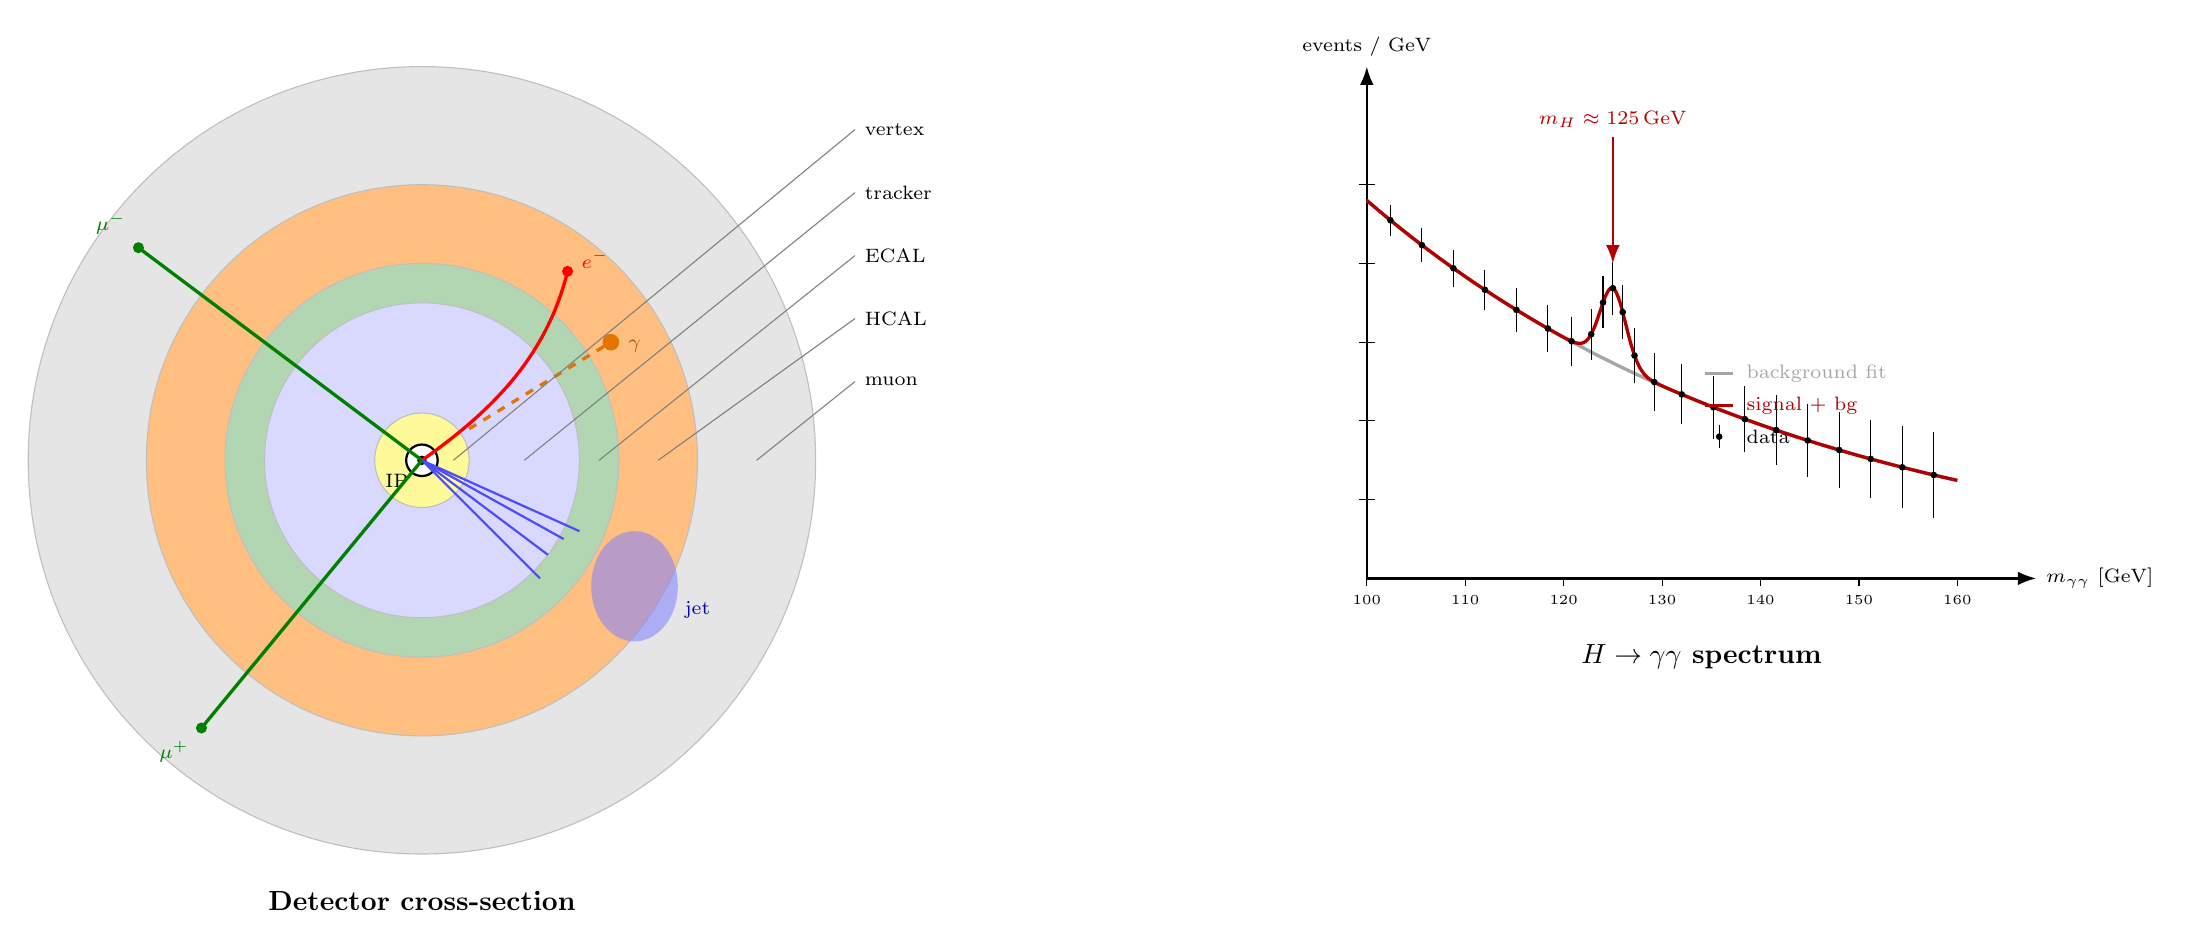
\begin{tikzpicture}[>=Latex,font=\small]

% =====================================================
% LEFT: Detector cross-section (onion)
% =====================================================
\begin{scope}[xshift=0cm,yshift=0cm]

% Five concentric layers (radii in cm chosen for visual clarity, not literal scale):
% beam pipe ~0.2, vertex 0.2-0.6, tracker 0.6-2.0, ECAL 2.0-2.5, HCAL 2.5-3.5, muon 3.5-5.0

% Muon chambers (outermost, light gray)
\fill[gray!20] (0,0) circle (5.0);
% HCAL (orange-red)
\fill[orange!50] (0,0) circle (3.5);
% ECAL (green)
\fill[green!45!black!30] (0,0) circle (2.5);
% Tracker (light blue)
\fill[blue!15] (0,0) circle (2.0);
% Vertex detector (light yellow)
\fill[yellow!40] (0,0) circle (0.6);
% Beam pipe (white center)
\fill[white] (0,0) circle (0.2);

% Layer outlines
\draw[gray!50,thin] (0,0) circle (5.0);
\draw[gray!50,thin] (0,0) circle (3.5);
\draw[gray!50,thin] (0,0) circle (2.5);
\draw[gray!50,thin] (0,0) circle (2.0);
\draw[gray!50,thin] (0,0) circle (0.6);
\draw[black,thick] (0,0) circle (0.2);

% Interaction point
\fill[black] (0,0) circle (0.06);
\node[anchor=north east,font=\scriptsize] at (-0.05,-0.05) {IP};

% --- Tracks from interaction point ---
% Electron (red solid, curved slightly, stops at ECAL)
\draw[red,very thick]
  (0,0) .. controls (1.0,0.7) and (1.6,1.4) .. (1.85,2.4);
\fill[red] (1.85,2.4) circle (2pt);
\node[red,font=\scriptsize] at (2.2,2.55) {$e^-$};

% Photon (orange dashed, no track inside tracker, deposit in ECAL)
\draw[orange!90!black,very thick,dashed]
  (0.6,0.4) -- (2.4,1.5);
\fill[orange!90!black] (2.4,1.5) circle (3pt);
\node[orange!70!black,font=\scriptsize] at (2.7,1.45) {$\gamma$};

% Hadronic jet (blue cone-like, several tracks ending in HCAL)
\draw[blue!70,thick] (0,0) -- (1.6,-1.2);
\draw[blue!70,thick] (0,0) -- (1.8,-1.0);
\draw[blue!70,thick] (0,0) -- (1.5,-1.5);
\draw[blue!70,thick] (0,0) -- (2.0,-0.9);
% Shower spread in HCAL
\fill[blue!50,opacity=0.55] (2.7,-1.6) ellipse (0.55 and 0.7);
\node[blue!70!black,font=\scriptsize] at (3.5,-1.9) {jet};

% Muon (green solid, straight, passes everything)
\draw[green!50!black,very thick]
  (0,0) -- (-3.6,2.7);
\fill[green!50!black] (-3.6,2.7) circle (2pt);
\node[green!50!black,font=\scriptsize] at (-3.95,3.0) {$\mu^-$};

% Another muon opposite direction for symmetry
\draw[green!50!black,very thick]
  (0,0) -- (-2.8,-3.4);
\fill[green!50!black] (-2.8,-3.4) circle (2pt);
\node[green!50!black,font=\scriptsize] at (-3.15,-3.7) {$\mu^+$};

% --- Layer labels (placed outside on the right side) ---
\draw[gray,thin] (0.4,0) -- (5.5,4.2);
\node[font=\scriptsize,anchor=west] at (5.5,4.2) {vertex};
\draw[gray,thin] (1.3,0) -- (5.5,3.4);
\node[font=\scriptsize,anchor=west] at (5.5,3.4) {tracker};
\draw[gray,thin] (2.25,0) -- (5.5,2.6);
\node[font=\scriptsize,anchor=west] at (5.5,2.6) {ECAL};
\draw[gray,thin] (3.0,0) -- (5.5,1.8);
\node[font=\scriptsize,anchor=west] at (5.5,1.8) {HCAL};
\draw[gray,thin] (4.25,0) -- (5.5,1.0);
\node[font=\scriptsize,anchor=west] at (5.5,1.0) {muon};

% Title
\node[font=\bfseries] at (0,-5.6) {Detector cross-section};

\end{scope}

% =====================================================
% RIGHT: m_gamma_gamma spectrum
% =====================================================
\begin{scope}[xshift=12cm,yshift=-1.5cm]

% Axes
\def\xmin{0}
\def\xmax{8.5}
\def\ymin{0}
\def\ymax{6.5}

\draw[->,thick] (0,0) -- (\xmax,0) node[right,font=\scriptsize] {$m_{\gamma\gamma}$ [GeV]};
\draw[->,thick] (0,0) -- (0,\ymax) node[above,font=\scriptsize] {events / GeV};

% X-axis ticks from 100 to 160 GeV
% mapping: 100 -> 0, 160 -> 7.5
\foreach \m/\x in {100/0,110/1.25,120/2.5,130/3.75,140/5.0,150/6.25,160/7.5}{
  \draw (\x,0) -- (\x,-0.1) node[below,font=\tiny] {\m};
}
% Y-axis ticks
\foreach \y in {1,2,3,4,5}{
  \draw (-0.1,\y) -- (0.1,\y);
}

% Smooth background curve: decreasing, sample points
% B(x) = 4.8 * exp(-0.18*x) at x in [0, 7.5]
\draw[gray!70,very thick,smooth,domain=0:7.5,samples=80,variable=\x]
  plot (\x, {4.8*exp(-0.18*\x)});

% Signal Gaussian peak at m=125 GeV -> x = 3.125, height ~ 1.05 (approx 30% of bg there)
% bg at 3.125 = 4.8*exp(-0.5625) ~ 2.74
% signal height: 0.85
% sigma in x units: 1.3 GeV / 8 GeV per unit = 0.1625
% Signal+bg curve (brick red)
\draw[red!70!black,very thick,smooth,domain=0:7.5,samples=120,variable=\x]
  plot (\x, {4.8*exp(-0.18*\x) + 0.95*exp(-((\x-3.125)*(\x-3.125))/(2*0.1625*0.1625))});

% Data points with error bars along the s+b curve
\foreach \x in {0.3,0.7,1.1,1.5,1.9,2.3,2.6,2.85,3.0,3.125,3.25,3.4,3.65,4.0,4.4,4.8,5.2,5.6,6.0,6.4,6.8,7.2}{
  \pgfmathsetmacro{\bgval}{4.8*exp(-0.18*\x)}
  \pgfmathsetmacro{\sigval}{0.95*exp(-((\x-3.125)*(\x-3.125))/(2*0.1625*0.1625))}
  \pgfmathsetmacro{\yval}{\bgval+\sigval}
  \pgfmathsetmacro{\err}{0.18+0.05*\x}
  \draw[black,thin] (\x,{\yval-\err}) -- (\x,{\yval+\err});
  \fill[black] (\x,\yval) circle (1.2pt);
}

% Arrow + label at 125 GeV
\draw[->,thick,red!70!black] (3.125,5.6) -- (3.125,4.0);
\node[red!70!black,font=\scriptsize,anchor=south] at (3.125,5.6) {$m_H \approx 125\,\mathrm{GeV}$};

% Legend
\node[gray!70,font=\scriptsize,anchor=west] at (4.7,2.6) {background fit};
\draw[gray!70,very thick] (4.3,2.6) -- (4.65,2.6);

\node[red!70!black,font=\scriptsize,anchor=west] at (4.7,2.2) {signal $+$ bg};
\draw[red!70!black,very thick] (4.3,2.2) -- (4.65,2.2);

\node[black,font=\scriptsize,anchor=west] at (4.7,1.8) {data};
\fill[black] (4.475,1.8) circle (1.2pt);
\draw[black,thin] (4.475,1.65) -- (4.475,1.95);

% Title
\node[font=\bfseries] at (\xmax/2,-1.0) {$H \to \gamma\gamma$ spectrum};

\end{scope}

\end{tikzpicture}
\end{document}
